На основе базового класса Pokemon написать свои классы для заданных видов покемонов. Каждый вид покемона должен иметь один или два типа и стандартные базовые характеристики:

\begin{itemize}
	\item очки здоровья (HP)
	\item атака (attack)
	\item защита (defense)
	\item специальная атака (special attack)
	\item специальная защита (special defense)
	\item скорость (speed)
\end{itemize}

Классы покемонов должны наследоваться в соответствии с цепочкой эволюции покемонов. На основе базовых классов PhysicalMove, SpecialMove и StatusMove реализовать свои классы для заданных видов атак. Все разработанные классы, не имеющие наследников, должны быть реализованы таким образом, чтобы от них нельзя было наследоваться.

Атака должна иметь стандартные тип, силу (power) и точность (accuracy). Должны быть реализованы стандартные эффекты атаки. Назначить каждому виду покемонов атаки в соответствии с вариантом. Уровень покемона выбирается минимально необходимым для всех реализованных атак.

Используя класс симуляции боя Battle, создать 2 команды покемонов (каждый покемон должен иметь имя) и запустить бой.

Базовые классы и симулятор сражения находятся в jar-архиве (обновлен 9.10.2018, исправлен баг с добавлением атак и кодировкой). Документация в формате javadoc - здесь.

Информацию о покемонах, цепочках эволюции и атаках можно найти на сайтах http://poke-universe.ru, http://pokemondb.net, http://veekun.com/dex/pokemon

\begin{figure}[h]
	\centering
	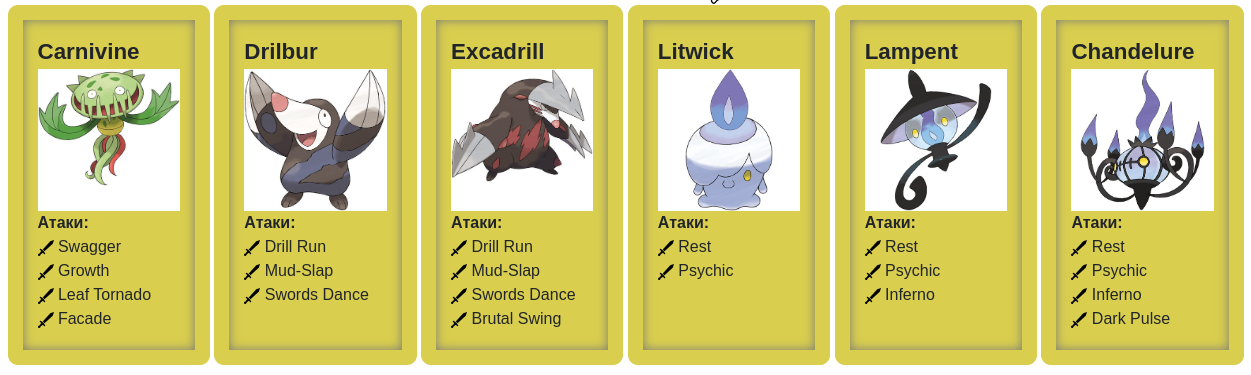
\includegraphics[scale=1.5]{pokemons}
\end{figure}